\section{Conditional Probability}

\begin{figure}[b]
	\centering
	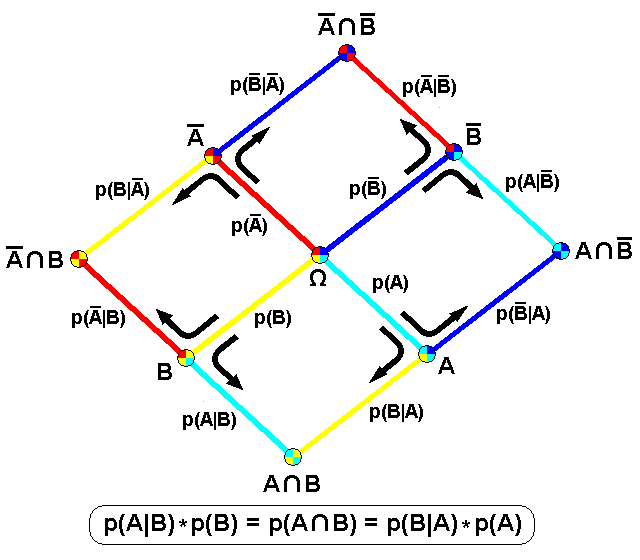
\includegraphics[width=0.7\linewidth]{images/Bayes_Theorem_2D}
	\caption{Diagram for Bayes' theorem.}
	\label{fig:2.4.1}
\end{figure}


In this section, we will review Bayes' theorem, which describes the probability of an event occurring based on prior knowledge of conditions related to the problem. 

To understand this theorem, we need to define conditional probability and how we can use the elements of a partition to calculate the probability of an event.


\begin{figure}
	\centering
	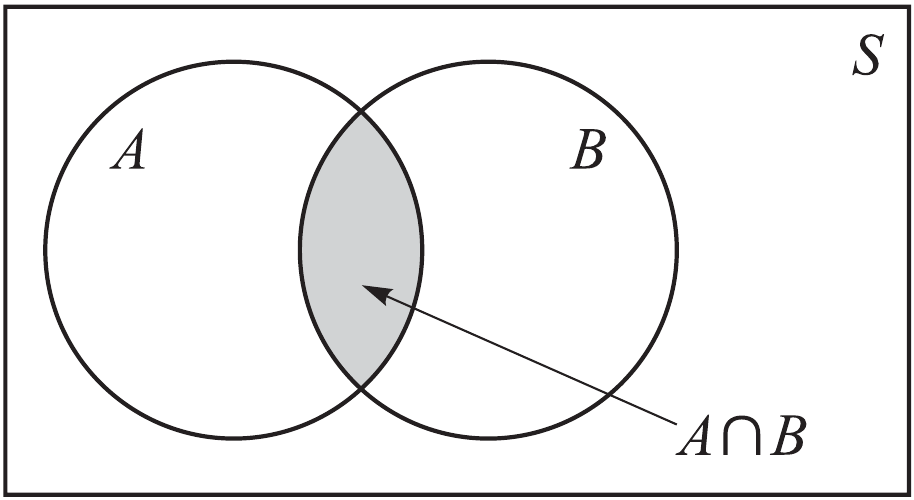
\includegraphics[width=5cm,keepaspectratio=true]{./pe/pands0103.png}
	% pands0103.png: 0x0 pixel, 300dpi, 0.00x0.00 cm, bb=
	\label{fig:2.4.2}
	\caption{Union of two sets}
\end{figure}

Let $A,B\subset S$ be two events such that $P(A)>0.$ We will denote by $P(B|A)$
the probability of $B$ given that $A$ has occurred, which is called the \emph{conditional probability} of $B$ given $A.$ Formally:


\begin{definition}[Conditional probability]
	\begin{align}
		P(B|A)&=\dfrac{P(A\cap B)}{P(A)} \\
		P(A\cap B) &= P(A)P(B|A)
	\end{align}
\end{definition}


\begin{remark}
	Conditional probability satisfies all the axioms of a probability function. We can think of $P(\cdot|A)$ as the probability function obtained by replacing the sample space $S$ with $A.$
\end{remark}

\begin{example}
	Five marbles are placed in a jar: three white and two black. Immediately afterwards, the jar is shaken to randomize its contents. Determine the probability that on the second draw we extract a black marble, given that on the first draw we obtained a white marble.  
\end{example}

\begin{solution}
	Let the event $ E_i $ consist of obtaining a white marble on the $i$-th attempt, so that $ E_i' $ represents obtaining a black marble. 
	
	Then, the probability of drawing a white marble first followed by a black marble is:
	\begin{align}
		P(E_1\cap E_2') = \dfrac{3}{5}\times \dfrac{2}{4}=\dfrac{6}{20}.
	\end{align}
	This is because on the first turn there are three white marbles out of five, but if we draw a white marble (without replacement), four marbles remain, two of which are white. 
	
	Now, the probability $ P(E_1) $ of drawing a white marble on the first attempt is $ \dfrac{3}{5} $, so that:
	\begin{align}
		P(E_2'|E_1) = \dfrac{1}{2}.
	\end{align}
\end{solution}





{}
\begin{theorem}
	\label{thm:2.4.1}
	For any three events $A_{1},A_{2},A_{3},$ we have
	\begin{align}
		\label{eq:2.4.1}
		P(A_{1} \cap A_{2} \cap A_{3})=P(A_{1})P(A_{2}|A_{1})P(A_{3}|A_{1} \cap A_{2})
	\end{align}
\end{theorem}


{}
\begin{theorem}
	\label{thm:2.4.2} If $S=A_{1}\sqcup ... \sqcup A_{N},$ then
	\begin{align}
		\label{eq:2.4.2}
		P(A)=P(A_{1})P(A|A_{1})+...+P(A_{N})P(A|A_{N})
	\end{align}
\end{theorem}


{}
If $P(B|A)=P(B),$ i.e., the probability of $B$ occurring is unaffected by the occurrence of $A,$ then we say that $A$ and $B$ are independent.


\begin{definition}
	$A$ and $B$ are independent events if and only if
	\begin{align}
		\label{eq:2.4.3}
		P(A \cap B) = P(A)P(B).
	\end{align}
\end{definition}


{}
This definition can be generalized to more than two events. For instance, we say that $A_{1},A_{2},A_{3}$ are independent events if
\begin{align}
	k\neq j \rightarrow P(A_{j} \cap A_{k})=P(A_{j})P(A_{k}), \; j,k=1,2,3 
	\\ P(A_{1}\cap A_{2} \cap A_{3})=P(A_{1})P(A_{2})P(A_{3}).
\end{align}


%\begin{theorem}[Bayes' Theorem]
%	If $S=A_{1}\sqcup A_{2} \sqcup...\sqcup A_{N},$ then
%	\begin{align}
%		\label{1.24}
%		P(A_{k}|A) = \dfrac{P(A_{k})P(A|A_{k})}{\sum_{j} P(A_{j})P(A|A_{j})}
%	\end{align}
%	
%\end{theorem}
